\section{Extended Taxonomy}
\label{sec:taxonomy}

The $3\times 3 \times 3$ taxonomy introduced by \citet{DBLP:journals/corr/abs-2512-13564} captures the design space of agent memory along three well-motivated axes: storage form, functional purpose, and lifecycle stage. It has proven durable enough to accommodate all 952 papers in our dataset. However, our analysis of the 498 papers published since February 2026---as well as re-examination of earlier works---reveals nine cross-cutting themes that the original axes do not explicitly surface. These themes span multiple taxonomy cells and represent distinct design considerations that are invisible when papers are classified solely by form, function, and dynamics.

In response, we propose three new orthogonal dimensions that augment the original taxonomy. These are additions, not replacements: a paper classified as Factual/Token-level/Formation retains that classification, but now additionally receives coordinates along the Temporal Dynamics, Modality, and Biological Inspiration axes. Figure~\ref{fig:taxonomy} visualizes the full extended taxonomy.

\subsection{Cross-Cutting Themes}

\textbf{Temporal Dynamics.} Over 130 papers now explicitly model how memory changes over time beyond the original Dynamics axis's lifecycle stages, up from a handful at the time of the original survey. \citet{Unknown2025Zep} introduces a temporal knowledge graph architecture that associates each fact with a timestamp and supports time-relative queries. \citet{Unknown2026FadeMem} proposes biologically inspired forgetting curves that decay memory importance over time, mirroring the Ebbinghaus forgetting curve. \citet{Unknown2026Engram} implements a bi-temporal memory engine that separately tracks when a memory was stored (transaction time) and when it describes (valid time), enabling temporal reasoning and retroactive updates. \citet{Unknown2026SCM} simulates NREM/REM sleep cycles to consolidate and prune memories offline. These works treat time not merely as an ordering mechanism but as a first-class dimension with decay, consolidation, and bi-temporal semantics.

\textbf{Multimodality.} Nearly 100 papers in our dataset handle memory for non-text modalities, a sharp increase from the fourteen identified at the original survey's cutoff. \citet{Unknown2025MemVerse} and \citet{Unknown2025WorldMM} build multimodal memory systems for vision and video. \citet{Unknown2026TeleMem} stores both textual and visual episodic memories for long-horizon tasks. \citet{Unknown2025VisMem} introduces a latent vision memory that stores visual features outside the LLM's hidden states. \citet{Unknown2025MemoryVLA} extends memory into the embodied domain with vision-language-action models for robotics. \citet{Unknown2025SeeingListeningRemem} integrates audio, vision, and text into a unified memory store. The original taxonomy's exclusive focus on text-based memory---implicit in its examples and subcategories---misses this dimension entirely.

\textbf{Graph and Structured Representations.} Approximately 100 papers organize memory as explicit graph structures, up from six at the original survey's cutoff. \citet{Unknown2026MAGMA} uses multi-graph architectures with separate graphs for semantic, episodic, and procedural knowledge. \citet{Unknown2025Zep} stores memory in a temporal knowledge graph. \citet{Unknown2026MRAgent} reconstructs memories as graph structures at retrieval time rather than storing flat vectors. \citet{Unknown2026Engram} combines knowledge graphs with bi-temporal indexing. \citet{Unknown2025SGMem} uses sentence-level graph representations to capture entity relationships. These works suggest that graph-structured memory is a distinct design choice with implications for expressiveness, queryability, and storage efficiency.

\textbf{Biologically and Neurocognitively Inspired.} Roughly 40 papers draw explicit inspiration from human memory systems. \citet{Unknown2026CraniMem} implements a cranial-inspired gating mechanism that bounds memory writes. \citet{Unknown2026FadeMem} models forgetting via biological decay functions. \citet{Unknown2026SCM} directly simulates hippocampal--neocortical consolidation through artificial sleep cycles. \citet{Unknown2026HumanInspiredMemoryA} models the dual-process theory of memory with separate fast-learning and slow-learning pathways. \citet{Unknown2026Engram} takes its name from the biological engram---the physical substrate of a memory trace. While earlier work like HippoRAG~\cite{Unknown2024HippoRAG} used the hippocampus as a loose metaphor, these newer systems engage much more deeply with cognitive and neuroscientific theory, meriting an explicit analytical dimension.

\textbf{Lifelong and Continual Learning.} Nearly 190 papers address the challenge of persistent, self-evolving memory that accumulates over unbounded interactions---the largest theme cluster in our dataset. \citet{Unknown2026AllMem} evolves memory topology dynamically as new experiences arrive. \citet{Unknown2026ContinuumMemoryArchi} proposes architectures that maintain a fixed memory budget while continuously integrating new information. \citet{Unknown2026MemRL} uses runtime reinforcement learning to update memory policies from interaction feedback. \citet{Unknown2025AgentEvolver} defines an agent evolution loop that refines both memory content and access strategies. These works extend beyond the original Dynamics axis's Evolution subtypes by tackling the open-ended nature of lifelong deployment.

\textbf{Benchmark and Evaluation.} Over 80 benchmark-focused papers reveal the field's growing demand for standardized evaluation, a more than fourfold increase since the original survey. \citet{Wu2024LongMemEval} evaluates chat assistants on long-term interactive memory. \citet{Tan2025MemBench} proposes comprehensive memory evaluation across multiple dimensions. \citet{Unknown2025MemoryAgentBench} uses incremental multi-turn interactions to isolate memory-specific from reasoning-specific capabilities. \citet{Unknown2026LongMemEvalV2} extends LongMemEval to the experiential memory domain. These benchmarks operate at different levels of granularity and cover different memory capabilities, but no single benchmark spans the full taxonomy---a gap we analyze in Section~\ref{sec:benchmarks}.

\textbf{Retrieval Fusion.} Approximately 30 papers combine multiple retrieval signals for improved memory access. \citet{Unknown2026MRAgent} reconstructs memory at retrieval time, fusing semantic similarity with graph traversal. \citet{Unknown2025Mem0} combines semantic search, BM25 keyword matching, and entity linking in a hybrid retrieval pipeline. \citet{Unknown2026Engram} uses both temporal and semantic retrieval signals. Retrieval fusion represents a distinct design pattern that the original taxonomy's Retrieval subtypes (Retrieval vs.\ Query Construction) do not fully capture.

\textbf{Security and Adversarial Robustness.} Over 120 papers now address the security of agent memory systems---a theme that was nascent at the time of the original survey and has since grown into one of the largest clusters in the field. These works study memory poisoning attacks, in which adversaries inject malicious content into persistent stores; prompt injection that persists across sessions via memory; stealthy memory corruption in recommender and personal agents; and defenses including provenance tracking, watermarking, and anomaly detection. Representative systems include AgentPoison~\cite{Unknown2025AgentPoison}, which red-teams memory and knowledge bases; MemPoison, which uncovers persistent memory threats; and MemMorph, which demonstrates tool hijacking via memory poisoning. The original taxonomy's trustworthiness discussion treated this as a future direction; the data now shows it as a first-class concern.

\textbf{Efficiency and Compression.} Approximately 140 papers address the efficiency of memory systems, focusing on KV-cache management, context compression, and token-budgeted retrieval. This theme is driven by the practical constraint that long-running agents cannot simply accumulate context indefinitely. Representative works include KV-cache compression for long-horizon GUI agents, training-free context management, and decision-aware memory cards that select and compress context for tool-using agents. While the original taxonomy's Working/Latent cell captures some of this activity, the scale and specificity of efficiency-focused work---much of it operating below the prompt level on attention mechanisms---warrants recognition as a distinct theme.

\subsection{Three New Dimensions}

Based on these nine themes, we propose three additional dimensions. Table~\ref{tab:dimensions} summarizes their levels and representative papers.

\subsubsection{Temporal Dynamics}

This dimension captures how a memory system models the passage of time and its effect on memory content. The levels are:

\begin{description}[nosep]
  \item[None.] The system does not model time beyond implicit ordering (e.g., FIFO eviction). Most pre-2025 token-level buffers fall here.
  \item[Decay-based.] Memory strength decreases over time according to a decay function, and weakened memories may be evicted or archived. Examples: FadeMem~\cite{Unknown2026FadeMem}, Mem0's recency-weighted retrieval~\cite{Unknown2025Mem0}.
  \item[Consolidation-based.] Memory undergoes offline processing---merging, abstracting, or pruning---at periodic intervals. Examples: SCM's sleep consolidation~\cite{Unknown2026SCM}, MemEvolve~\cite{Unknown2025MemEvolve}.
  \item[Bi-temporal.] The system tracks both transaction time (when stored) and valid time (when described), enabling temporal queries and retroactive updates. Examples: Engram~\cite{Unknown2026Engram}, Zep~\cite{Unknown2025Zep}.
\end{description}

\subsubsection{Modality}

This dimension captures the sensory channels a memory system handles:

\begin{description}[nosep]
  \item[Text-only.] Memory stores and retrieves textual information only. The majority of papers in our dataset (approximately 89\%) fall into this level, though the multimodal share has grown from 7\% to roughly 10\% as the corpus expanded.
  \item[Multimodal-in.] Memory accepts non-text inputs (images, video, audio) but stores and retrieves textual descriptions or summaries. Examples: MemVerse~\cite{Unknown2025MemVerse}, WorldMM~\cite{Unknown2025WorldMM}.
  \item[Multimodal-out.] Memory stores non-text representations (visual features, audio embeddings) and retrieves them for downstream tasks. Examples: VisMem~\cite{Unknown2025VisMem}, MemoryVLA~\cite{Unknown2025MemoryVLA}, TeleMem~\cite{Unknown2026TeleMem}.
  \item[Full-multimodal.] Memory operates across text, vision, audio, and embodiment simultaneously with cross-modal retrieval. Examples: Seeing/Listening/Remembering/Reasoning~\cite{Unknown2025SeeingListeningRemem}, Embodied VideoAgent~\cite{Unknown2025EmbodiedVideoAgent}.
\end{description}

\subsubsection{Biological Inspiration}

This dimension captures how deeply a memory system engages with biological cognition:

\begin{description}[nosep]
  \item[None.] No explicit biological inspiration. The system is designed purely from an engineering perspective.
  \item[Cognitive-metaphor.] The system uses high-level cognitive concepts (e.g., ``episodic memory,'' ``consolidation'') as loose metaphors without detailed biological fidelity. Most experiential memory systems fall here.
  \item[Neuro-inspired.] The system explicitly models neuroscientific mechanisms (e.g., forgetting curves, hippocampal indexing, synaptic gating) but does not attempt full biological fidelity. Examples: HippoRAG~\cite{Unknown2024HippoRAG}, FadeMem~\cite{Unknown2026FadeMem}, CraniMem~\cite{Unknown2026CraniMem}.
  \item[Brain-architecture.] The system implements a detailed computational model of a brain subsystem, including multiple interacting regions or cell types. Examples: SCM's sleep-consolidated memory~\cite{Unknown2026SCM}, Human-Inspired~\cite{Unknown2026HumanInspiredMemoryA}, XMem's Atkinson--Shiffrin model~\cite{Unknown2022XMem}.
\end{description}

\begin{table}[ht]
    \centering
    \caption{Three new orthogonal taxonomy dimensions with their levels.}
    \label{tab:dimensions}
    \small
    \begin{tabular}{lll}
        \toprule
        \textbf{Dimension} & \textbf{Levels} & \textbf{Description} \\
        \midrule
        Temporal Dynamics & None, Decay, Consolidation, Bi-temporal & How memory changes over time \\
        Modality & Text, M.-in, M.-out, Full & Data modalities memory handles \\
        Biological Inspiration & None, Cognitive, Neuro, Brain & Fidelity to biological cognition \\
        \bottomrule
    \end{tabular}
\end{table}

\begin{figure}[ht]
    \centering
    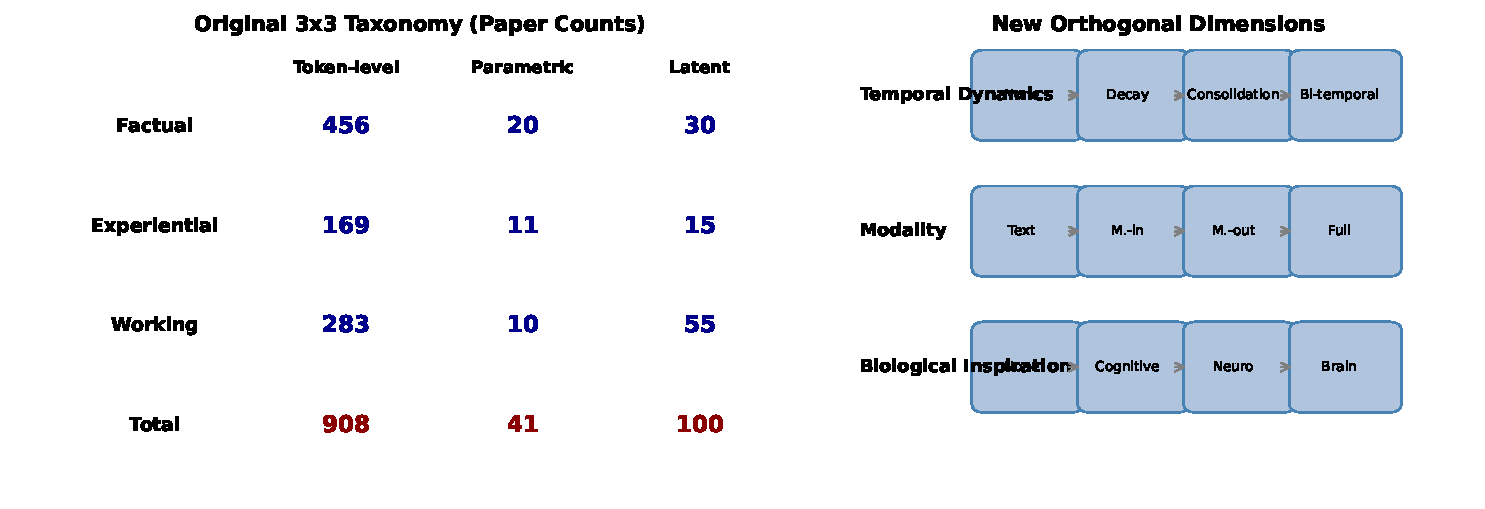
\includegraphics[width=0.95\textwidth]{figures/fig1_taxonomy.pdf}
    \caption{Left: Paper counts across the original 3x3 taxonomy. Right: Structure of three new orthogonal dimensions.}
    \label{fig:taxonomy}
\end{figure}

\subsection{Impact on Taxonomy Coverage}

Figure~\ref{fig:heatmap} shows the distribution of papers across the original $3\times 3 \times 3$ cells, overlaid with the new dimensions. The addition of the three new axes reveals previously invisible structure. For example, the Experiential/Token-level cell, which contains 153 papers, spans all four levels of the Biological Inspiration dimension---most are Cognitive-metaphor, but FadeMem (Neuro-inspired) and SCM (Brain-architecture) represent qualitatively different approaches within the same form--function cell.

The extended taxonomy does not change the number of papers assigned to any original cell; rather, it adds resolution within each cell and enables cross-cell analyses along the new axes. For instance, it reveals that multimodal memory is concentrated in Working/Latent (VisMem, MemoryVLA, Time-VLM~\cite{Unknown2025TimeVLM}) and Factual/Token-level (MemVerse, WorldMM), leaving other cells underexplored---a pattern invisible in the original taxonomy.

\subsection{Methodological Note}

The assignment of new-dimension levels to papers is itself a data-driven process. We analyzed the 952 papers in \texttt{papers.yaml}, reading abstracts and, where necessary, full texts to determine the three additional coordinates. The resulting annotations are included in the data file for community verification and improvement. We expect these annotations to evolve as the field matures; the data-driven infrastructure described in Section~\ref{sec:methodology} is designed to accommodate such changes.

\begin{figure}[ht]
    \centering
    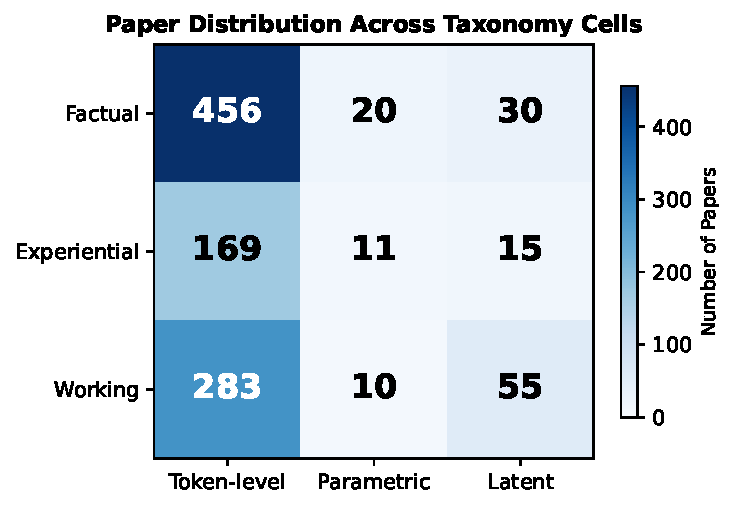
\includegraphics[width=0.65\textwidth]{figures/fig2_heatmap.pdf}
    \caption{Heatmap of paper distribution across the 3x3 taxonomy cells. Darker colors indicate higher concentration of research activity.}
    \label{fig:heatmap}
\end{figure}
